\documentclass[11pt]{article}
\usepackage{cornell-notes}
\usepackage{mathtools}
\usepackage{needspace}
\usepackage{ragged2e}
\usepackage{adjustbox}
\usepackage{tikz}
\usetikzlibrary{arrows.meta,positioning}
\tcbuselibrary{most}
\geometry{letterpaper,margin=0.72in,headheight=15pt}
\setCornellCollection{Calculus Cornell Notes}
\setCornellUnitType{Chapter}
\setCornellUnitNumber{1}
\setCornellUnitTitle{Limits and Their Properties}

\definecolor{Ink}{HTML}{17324D}
\definecolor{Teal}{HTML}{147D78}
\definecolor{Sky}{HTML}{DDEEF1}
\definecolor{Cue}{HTML}{EEF2F5}
\definecolor{Warm}{HTML}{FFF3D6}
\definecolor{Alert}{HTML}{9D3C32}
\definecolor{Green}{HTML}{276749}
\definecolor{Rule}{HTML}{AAB8C2}
\hypersetup{colorlinks=true,linkcolor=Ink,urlcolor=Teal,pdfborder={0 0 0}}
\setlength{\parindent}{0pt}
\setlength{\parskip}{4pt}
\setlist{nosep,leftmargin=*}
\titleformat{\section}{\Large\bfseries\color{Ink}}{}{0pt}{}[\color{Teal}\titlerule]
\titleformat{\subsection}{\large\bfseries\color{Teal}}{}{0pt}{}
\pagestyle{fancy}
\fancyhf{}
\fancyhead[L]{\small\color{Ink}\textsc{Cornell Notes}}
\fancyhead[R]{\small\color{Teal}\nouppercase{\leftmark}}
\fancyfoot[L]{\footnotesize\color{Ink}Active recall $\bullet$ Worked reasoning $\bullet$ Verification}
\fancyfoot[R]{\footnotesize\color{Ink}\thepage\ of \pageref*{LastPage}}
\renewcommand{\headrulewidth}{0.5pt}
\renewcommand{\footrulewidth}{0.4pt}
\newcolumntype{Y}{>{\RaggedRight\arraybackslash}X}
\newtcolorbox{orientationbox}{enhanced,breakable,colback=Sky,colframe=Teal,boxrule=0.7pt,arc=2mm,title=Chapter orientation,fonttitle=\bfseries}
\newtcolorbox{sectionsummarybox}{enhanced,breakable,colback=white,colframe=Teal,boxrule=0.6pt,arc=1.5mm,left=2mm,right=2mm,top=1mm,bottom=1mm,title=Section synthesis,fonttitle=\bfseries\color{Teal}}
\newtcolorbox{warningbox}{enhanced,breakable,colback=Warm,colframe=Alert,boxrule=0.7pt,arc=1.5mm,title=Common error audit,fonttitle=\bfseries}
\newtcolorbox{checkbox}{enhanced,breakable,colback=white,colframe=Green,boxrule=0.7pt,arc=1.5mm,title=Verification habit,fonttitle=\bfseries}
\newcommand{\cornellcuehead}{\rowcolor{Ink}\color{white}\bfseries Cue / recall prompt & \color{white}\bfseries Notes / reasoning \\\endhead}
\newcommand{\cornellcuerow}[2]{\rowcolor{Cue}#1 & #2 \\\addlinespace[3pt]}
% Table-safe: delegates to the shared Cornell formula box (cornell-notes.sty),
% which cannot emit \pagebreak/\noalign inside longtable cells.
\newcommand{\formula}[1]{\CornellFormula[colback=Sky,colframe=Teal]{#1}}

\title{Chapter 1: Limits and Their Properties\\[2mm]\large Cornell Notes}
\author{}
\date{}
\hypersetup{pdftitle={Chapter 1: Limits and Their Properties - Cornell Notes},pdfauthor={},pdfsubject={Calculus study notes},pdfkeywords={calculus, Cornell notes, active recall}}
\begin{document}
\maketitle
\thispagestyle{fancy}
\begin{orientationbox}
Develop limits as the language of local behavior and use them to define continuity, infinite behavior, and the foundations of calculus. These notes follow the complete local section sequence (45--98) and emphasize definitions, governing results, strategy selection, and verifiable reasoning.
\end{orientationbox}

\section{Prerequisite map}
\begin{minipage}[t]{0.42\textwidth}
\textbf{Bring forward}
\begin{itemize}
\item Function graphs
\item Factoring and rationalization
\item Piecewise functions
\item Trigonometric identities
\end{itemize}
\end{minipage}\hfill
\begin{minipage}[t]{0.54\textwidth}
\textbf{Chapter flow}
\begin{center}
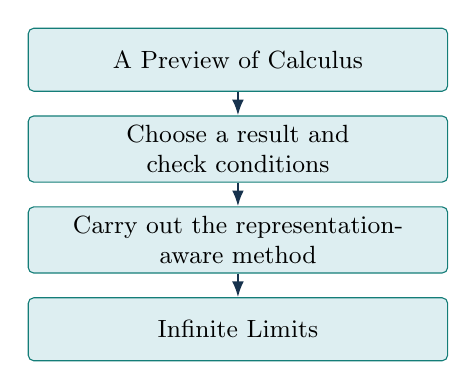
\begin{tikzpicture}[node distance=3mm, every node/.style={font=\small,align=center}, box/.style={draw=Teal,rounded corners=2pt,fill=Sky,minimum height=8mm,text width=0.42\textwidth}, arr/.style={-{Latex[length=2mm]},thick,draw=Ink}]
\node[box] (a) {A Preview of Calculus};
\node[box,below=of a] (b) {Choose a result and check conditions};
\node[box,below=of b] (c) {Carry out the representation-aware method};
\node[box,below=of c] (d) {Infinite Limits};
\draw[arr] (a)--(b); \draw[arr] (b)--(c); \draw[arr] (c)--(d);
\end{tikzpicture}
\end{center}
\end{minipage}

\section{Learning objectives}
\begin{enumerate}
\item Explain the central objects and hypotheses in 1.1 and 1.5.
\item Translate among algebraic, graphical, numerical, and verbal representations.
\item Select an appropriate formula or theorem before beginning symbolic work.
\item Carry out multi-step calculations while preserving domain, sign, orientation, and units.
\item Diagnose common errors by testing assumptions and checking the result independently.
\item Synthesize the chapter's methods into a reusable problem-solving workflow.
\end{enumerate}

\section{1.1 A Preview of Calculus}
\begin{longtable}{C N}\cornellcuehead
\cornellcuerow{What is the governing idea in 1.1?}{Tangent, velocity, area, and accumulation problems are linked by limiting processes that replace finite approximations with exact values.}
\cornellcuerow{Which result should be recalled?}{\formula{m_{\mathrm{tan}}=\lim_{h\to0}\frac{f(a+h)-f(a)}{h}}}
\cornellcuerow{How should a problem be organized?}{Translate the geometric or physical question into an approximating quantity, identify the refinement parameter, and describe its limiting value.}
\cornellcuerow{What should be checked before accepting an answer?}{Confirm the hypotheses and domain, preserve units and orientation when relevant, and substitute or differentiate back into the defining relation.}
\end{longtable}
\begin{warningbox}Treating a small approximation as exact obscures the limiting argument and its assumptions.\end{warningbox}
\begin{sectionsummarybox}Tangent, velocity, area, and accumulation problems are linked by limiting processes that replace finite approximations with exact values. The operational habit is to translate the geometric or physical question into an approximating quantity, identify the refinement parameter, and describe its limiting value.\end{sectionsummarybox}
\section{1.2 Finding Limits Graphically and Numerically}
\begin{longtable}{C N}\cornellcuehead
\cornellcuerow{What is the governing idea in 1.2?}{A limit describes the value approached by function outputs near an input, whether or not the function is defined there.}
\cornellcuerow{Which result should be recalled?}{\formula{\lim_{x\to a}f(x)=L}}
\cornellcuerow{How should a problem be organized?}{Approach from both sides with a graph and a table, compare the trends, and distinguish the limit from the actual value $f(a)$.}
\cornellcuerow{What should be checked before accepting an answer?}{Confirm the hypotheses and domain, preserve units and orientation when relevant, and substitute or differentiate back into the defining relation.}
\end{longtable}
\begin{warningbox}A coarse table, misleading graph window, or agreement from only one side does not establish a two-sided limit.\end{warningbox}
\begin{sectionsummarybox}A limit describes the value approached by function outputs near an input, whether or not the function is defined there. The operational habit is to approach from both sides with a graph and a table, compare the trends, and distinguish the limit from the actual value $f(a)$.\end{sectionsummarybox}
\section{1.3 Evaluating Limits Analytically}
\begin{longtable}{C N}\cornellcuehead
\cornellcuerow{What is the governing idea in 1.3?}{Limit laws reduce many problems to substitution after algebra exposes removable factors or standard limiting forms.}
\cornellcuerow{Which result should be recalled?}{\formula{\lim_{x\to0}\frac{\sin x}{x}=1,\qquad \lim_{x\to a}[f(x)+g(x)]=L+M}}
\cornellcuerow{How should a problem be organized?}{Try direct substitution, classify any indeterminate form, simplify by factoring or rationalizing, and then re-evaluate the equivalent expression.}
\cornellcuerow{What should be checked before accepting an answer?}{Confirm the hypotheses and domain, preserve units and orientation when relevant, and substitute or differentiate back into the defining relation.}
\end{longtable}
\begin{warningbox}Canceling a factor without noting the excluded point, or interpreting $0/0$ as a value, breaks the logic.\end{warningbox}
\begin{sectionsummarybox}Limit laws reduce many problems to substitution after algebra exposes removable factors or standard limiting forms. The operational habit is to try direct substitution, classify any indeterminate form, simplify by factoring or rationalizing, and then re-evaluate the equivalent expression.\end{sectionsummarybox}
\section{1.4 Continuity and One-Sided Limits}
\begin{longtable}{C N}\cornellcuehead
\cornellcuerow{What is the governing idea in 1.4?}{Continuity at $a$ requires a defined value, an existing two-sided limit, and equality between them; endpoint and piecewise behavior uses one-sided limits.}
\cornellcuerow{Which result should be recalled?}{\formula{f\text{ continuous at }a\iff \lim_{x\to a}f(x)=f(a)}}
\cornellcuerow{How should a problem be organized?}{Check left limit, right limit, and function value separately; use the Intermediate Value Theorem only on a continuous closed interval.}
\cornellcuerow{What should be checked before accepting an answer?}{Confirm the hypotheses and domain, preserve units and orientation when relevant, and substitute or differentiate back into the defining relation.}
\end{longtable}
\begin{warningbox}Matching a formula at the point is not enough if the neighboring values approach something else.\end{warningbox}
\begin{sectionsummarybox}Continuity at $a$ requires a defined value, an existing two-sided limit, and equality between them; endpoint and piecewise behavior uses one-sided limits. The operational habit is to check left limit, right limit, and function value separately; use the Intermediate Value Theorem only on a continuous closed interval.\end{sectionsummarybox}
\section{1.5 Infinite Limits}
\begin{longtable}{C N}\cornellcuehead
\cornellcuerow{What is the governing idea in 1.5?}{An infinite limit reports unbounded magnitude near an input and signals a vertical asymptote rather than a finite limit.}
\cornellcuerow{Which result should be recalled?}{\formula{\lim_{x\to a^+}f(x)=+\infty}}
\cornellcuerow{How should a problem be organized?}{Inspect signs on both sides of the candidate denominator zero, compare dominant local factors, and report each one-sided behavior.}
\cornellcuerow{What should be checked before accepting an answer?}{Confirm the hypotheses and domain, preserve units and orientation when relevant, and substitute or differentiate back into the defining relation.}
\end{longtable}
\begin{warningbox}Writing $\infty$ as though it were an ordinary real-number output leads to invalid arithmetic.\end{warningbox}
\begin{sectionsummarybox}An infinite limit reports unbounded magnitude near an input and signals a vertical asymptote rather than a finite limit. The operational habit is to inspect signs on both sides of the candidate denominator zero, compare dominant local factors, and report each one-sided behavior.\end{sectionsummarybox}

\section{Definitions and theorem register}
\small
\begin{longtable}{@{}>{\RaggedRight\arraybackslash}p{0.24\textwidth}>{\RaggedRight\arraybackslash}p{0.40\textwidth}>{\RaggedRight\arraybackslash}p{0.29\textwidth}@{}}
\toprule
\textbf{Topic} & \textbf{Meaning and conditions} & \textbf{Canonical form}\\
\midrule\endhead
1.1 A Preview of Calculus & Tangent, velocity, area, and accumulation problems are linked by limiting processes that replace finite approximations with exact values. & \adjustbox{max width=\linewidth}{\(\displaystyle m_{\mathrm{tan}}=\lim_{h\to0}\frac{f(a+h)-f(a)}{h}\)} \\\addlinespace[2pt]
1.2 Finding Limits Graphically and Numerically & A limit describes the value approached by function outputs near an input, whether or not the function is defined there. & \adjustbox{max width=\linewidth}{\(\displaystyle \lim_{x\to a}f(x)=L\)} \\\addlinespace[2pt]
1.3 Evaluating Limits Analytically & Limit laws reduce many problems to substitution after algebra exposes removable factors or standard limiting forms. & \adjustbox{max width=\linewidth}{\(\displaystyle \lim_{x\to0}\frac{\sin x}{x}=1,\qquad \lim_{x\to a}[f(x)+g(x)]=L+M\)} \\\addlinespace[2pt]
1.4 Continuity and One-Sided Limits & Continuity at $a$ requires a defined value, an existing two-sided limit, and equality between them; endpoint and piecewise behavior uses. & \adjustbox{max width=\linewidth}{\(\displaystyle f\text{ continuous at }a\iff \lim_{x\to a}f(x)=f(a)\)} \\\addlinespace[2pt]
1.5 Infinite Limits & An infinite limit reports unbounded magnitude near an input and signals a vertical asymptote rather than a finite limit. & \adjustbox{max width=\linewidth}{\(\displaystyle \lim_{x\to a^+}f(x)=+\infty\)} \\\addlinespace[2pt]
\bottomrule
\end{longtable}
\normalsize

\section{Formula and method sheet}
\small
\begin{longtable}{@{}>{\RaggedRight\arraybackslash}p{0.08\textwidth}>{\RaggedRight\arraybackslash}p{0.48\textwidth}>{\RaggedRight\arraybackslash}p{0.37\textwidth}@{}}
\toprule
\textbf{Sec.} & \textbf{Method sequence} & \textbf{Stop-and-check trigger}\\
\midrule\endhead
1.1 & Translate the geometric or physical question into an approximating quantity, identify the refinement parameter, and describe its limiting value. & Treating a small approximation as exact obscures the limiting argument and its assumptions. \\\addlinespace[2pt]
1.2 & Approach from both sides with a graph and a table, compare the trends, and distinguish the limit from the actual value $f(a)$. & A coarse table, misleading graph window, or agreement from only one side does not establish a two-sided limit. \\\addlinespace[2pt]
1.3 & Try direct substitution, classify any indeterminate form, simplify by factoring or rationalizing, and then re-evaluate the equivalent expression. & Canceling a factor without noting the excluded point, or interpreting $0/0$ as a value, breaks the logic. \\\addlinespace[2pt]
1.4 & Check left limit, right limit, and function value separately; use the Intermediate Value Theorem only on a continuous closed interval. & Matching a formula at the point is not enough if the neighboring values approach something else. \\\addlinespace[2pt]
1.5 & Inspect signs on both sides of the candidate denominator zero, compare dominant local factors, and report each one-sided behavior. & Writing $\infty$ as though it were an ordinary real-number output leads to invalid arithmetic. \\\addlinespace[2pt]
\bottomrule
\end{longtable}
\normalsize

\section{Common errors and diagnostic checks}
\begin{warningbox}
\begin{itemize}
\item \textbf{1.1:} Treating a small approximation as exact obscures the limiting argument and its assumptions.
\item \textbf{1.2:} A coarse table, misleading graph window, or agreement from only one side does not establish a two-sided limit.
\item \textbf{1.3:} Canceling a factor without noting the excluded point, or interpreting $0/0$ as a value, breaks the logic.
\item \textbf{1.4:} Matching a formula at the point is not enough if the neighboring values approach something else.
\item \textbf{1.5:} Writing $\infty$ as though it were an ordinary real-number output leads to invalid arithmetic.
\end{itemize}
\end{warningbox}
\begin{checkbox}
Before accepting any result: state the relevant domain; check theorem hypotheses; estimate sign and scale; preserve units and orientation; and verify by substitution, differentiation, a limiting case, or a second representation.
\end{checkbox}

\section{Chapter synthesis}
Develop limits as the language of local behavior and use them to define continuity, infinite behavior, and the foundations of calculus. The chapter begins with \textbf{A Preview of Calculus} and culminates in \textbf{Infinite Limits}. Across the sequence, the most reliable workflow is to identify the mathematical object, choose a representation, state the governing result with its hypotheses, compute without dropping restrictions, and audit the answer against the original definition. A limit is a claim about nearby behavior, so every evaluation must respect side, domain, algebraic equivalence, and the difference between approaching and attaining.

\section{Self-test questions}
\begin{enumerate}
\item Explain the central distinction or object in 1.1, using both words and notation.
\item State the main formula or result from 1.2 and identify every hypothesis or restriction needed for its use.
\item Describe the problem-solving procedure for 1.3. What is the strongest independent check?
\item Compare the roles of A Preview of Calculus and Infinite Limits within this chapter.
\item Reconstruct the governing formula for 1.4 from its geometric or analytic meaning.
\item Choose one method in the chapter and explain how its output should be interpreted, including units or orientation when applicable.
\item Scenario: A student working on 1.1 produces a polished calculation but makes this error: Treating a small approximation as exact obscures the limiting argument and its assumptions. Diagnose the earliest invalid step and repair the workflow.
\item Scenario: A solution in 1.2 quotes the displayed formula without checking conditions. Which conditions must be checked, and what could fail if they are absent?
\item Construct a concept map linking a representation, a governing result, a computation, and a verification check from this chapter.
\item Design a two-part test for mastery: one conceptual prompt and one calculation. State what evidence would count as a complete answer.
\end{enumerate}

\Needspace{8\baselineskip}
\section{Answer key}
\small
\begin{enumerate}
\item A complete response identifies Tangent, velocity, area, and accumulation problems are linked by limiting processes that replace finite approximations with exact values. It should connect that meaning to \(m_{\mathrm{tan}}=\lim_{h\to0}\frac{f(a+h)-f(a)}{h}\) and state the relevant domain.
\item The organizing result is \(\lim_{x\to a}f(x)=L\). The solver must check that the quantities are defined and that the assumptions named in 1.2 hold before applying it.
\item Use this sequence: Try direct substitution, classify any indeterminate form, simplify by factoring or rationalizing, and then re-evaluate the equivalent expression. The strongest check is to return to the defining relation or differentiate/substitute the result, as appropriate.
\item A Preview of Calculus establishes tangent, velocity, area, and accumulation problems are linked by limiting processes that replace finite approximations with exact values. Infinite Limits extends the chapter to an infinite limit reports unbounded magnitude near an input and signals a vertical asymptote rather than a finite limit. The connection is the reuse of the same representations under a broader method.
\item The formula \(f\text{ continuous at }a\iff \lim_{x\to a}f(x)=f(a)\) follows by translating the defining geometric or rate relationship into symbols; each factor records a distinct change or scale.
\item Interpretation must name what varies, with respect to what, and on which domain. A numerical value without units, sign, direction, or interval information is incomplete whenever those features are part of the modeled quantity.
\item The earliest fault is the unverified assumption described by this warning: Treating a small approximation as exact obscures the limiting argument and its assumptions. Restart by following this procedure: Translate the geometric or physical question into an approximating quantity, identify the refinement parameter, and describe its limiting value.
\item The formula \(\lim_{x\to a}f(x)=L\) is conditional, not decorative. Check domain, differentiability or integrability as relevant, boundary or orientation requirements, and nonzero denominators before drawing a conclusion.
\item One valid map is: the representation in 1.1 identifies the object; the result in 1.2 supplies a rule; the method in 1.3 carries out the computation; the check in 1.5 tests the conclusion against its definition.
\item The conceptual prompt should require explanation of a definition and its hypotheses. The calculation should require method selection rather than direct substitution. Full evidence includes setup, justified transformations, a result, and an independent check.
\end{enumerate}
\normalsize

\section{Key-term recap}
\small
\begin{longtable}{@{}>{\RaggedRight\arraybackslash}p{0.29\textwidth}>{\RaggedRight\arraybackslash}p{0.64\textwidth}@{}}
\toprule
\textbf{Term} & \textbf{Working meaning}\\
\midrule\endhead
A Preview of Calculus & Tangent, velocity, area, and accumulation problems are linked by limiting processes that replace finite approximations with exact values. \\\addlinespace[2pt]
Finding Limits Graphically and Numerically & A limit describes the value approached by function outputs near an input, whether or not the function is defined there. \\\addlinespace[2pt]
Evaluating Limits Analytically & Limit laws reduce many problems to substitution after algebra exposes removable factors or standard limiting forms. \\\addlinespace[2pt]
Continuity and One-Sided Limits & Continuity at $a$ requires a defined value, an existing two-sided limit, and equality between them; endpoint and piecewise behavior uses one-sided limits. \\\addlinespace[2pt]
Infinite Limits & An infinite limit reports unbounded magnitude near an input and signals a vertical asymptote rather than a finite limit. \\\addlinespace[2pt]
\bottomrule
\end{longtable}
\normalsize

\enlargethispage{4\baselineskip}
\begin{tcolorbox}[title=One-sentence takeaway,fonttitle=\bfseries,colback=Ink,colframe=Ink,coltext=white,coltitle=white,arc=2mm,boxrule=0pt]
\centering\bfseries A limit is a claim about nearby behavior, so every evaluation must respect side, domain, algebraic equivalence, and the difference between approaching and attaining.
\end{tcolorbox}
\end{document}
